Chương này trình bày các nền tảng lý thuyết liên quan đến đề tài, bao gồm tổng quan về Internet vạn vật (\ac{iot}), các mối đe dọa an ninh trong hệ thống \ac{iot}, và vai trò của hệ thống phát hiện xâm nhập (\ac{ids}). Bên cạnh đó, trong chương này, luận văn cũng giới thiệu kiến trúc và khả năng của Apache Spark trong xử lý dữ liệu lớn, các kỹ thuật học máy ứng dụng trong phát hiện bất thường và cách Spark MLlib hỗ trợ xây dựng mô hình học máy phân tán. Cuối cùng, chương đề cập đến một số nghiên cứu liên quan nhằm làm rõ khoảng trống mà luận văn hướng đến giải quyết.

\section{Tổng quan về \ac{iot}}
Internet of Things (\ac{iot}) là mạng lưới các thiết bị vật lý được tích hợp cảm biến, phần mềm và khả năng kết nối mạng, cho phép thu thập và trao đổi dữ liệu qua Internet \cite{Atzori2010}. \ac{iot} bao gồm các thiết bị như cảm biến môi trường, thiết bị gia dụng thông minh và phương tiện giao thông tạo ra khối lượng dữ liệu lớn với đặc điểm đa dạng, tốc độ cao và yêu cầu xử lý thời gian thực. Theo Cisco (2023), số lượng thiết bị \ac{iot} toàn cầu dự kiến đạt 29,4 tỷ vào năm 2030, nhấn mạnh tầm quan trọng của bảo mật trong lĩnh vực này \cite{Cisco2023}. Kiến trúc \ac{iot} thường được chia thành ba tầng:
\begin{itemize}
  \item \textbf{Tầng nhận thức}: Thu thập dữ liệu từ cảm biến và thiết bị.
  \item \textbf{Tầng mạng}: Truyền tải dữ liệu qua các giao thức như MQTT, CoAP hoặc HTTP.
  \item \textbf{Tầng ứng dụng}: Phân tích dữ liệu để cung cấp dịch vụ \cite{Khan2012}.
\end{itemize}

Tuy nhiên, các thiết bị \ac{iot} thường có tài nguyên hạn chế (bộ nhớ, năng lượng, khả năng tính toán), dẫn đến thách thức trong việc triển khai các giải pháp bảo mật truyền thống. Các mối đe dọa như tấn công từ chối dịch vụ (DDoS), tấn công giả mạo và khai thác lỗ hổng giao thức đòi hỏi các giải pháp bảo mật tiên tiến như \ac{ids}~\cite{HaddadPajouh2021}.

\section{Hệ thống phát hiện xâm nhập (\ac{ids})}
Hệ thống phát hiện xâm nhập (\ac{ids}) giám sát và phân tích hoạt động mạng hoặc hệ thống để phát hiện các hành vi bất thường hoặc đáng ngờ, nhằm bảo vệ hệ thống khỏi các cuộc tấn công mạng \cite{Liao2013}. \ac{ids} đóng vai trò quan trọng trong việc đảm bảo tính bảo mật, toàn vẹn và sẵn sàng của hệ thống \ac{iot}. \ac{ids} được phân loại như sau:

\textbf{Dựa trên vị trí triển khai:}
\begin{itemize}
  \item \textbf{Network-based \ac{ids} (NIDS)}: Giám sát lưu lượng mạng để phát hiện các mẫu tấn công.
  \item \textbf{Host-based \ac{ids} (HIDS)}: Tập trung vào hoạt động của một thiết bị cụ thể.
\end{itemize}

\vspace{1em}

\textbf{Dựa trên phương pháp phát hiện:}
\begin{itemize}
  \item \textbf{Signature-based \ac{ids}}: Sử dụng các mẫu tấn công đã biết, hiệu quả với các mối đe dọa quen thuộc nhưng hạn chế với các tấn công mới.
  \item \textbf{Anomaly-based \ac{ids}}: Phát hiện hành vi bất thường dựa trên mô hình hoạt động bình thường, phù hợp với các cuộc tấn công chưa biết.
  \item \textbf{Hybrid \ac{ids}}: Kết hợp cả hai phương pháp để tăng độ chính xác \cite{Bhadauria2012}.
\end{itemize}

Trong \ac{iot}, \ac{ids} phải xử lý khối lượng dữ liệu lớn và đáp ứng yêu cầu thời gian thực, đồng thời phù hợp với tài nguyên hạn chế của thiết bị. Các giải pháp \ac{ids} dựa trên dữ liệu lớn và học máy, như sử dụng Apache Spark, là hướng đi tiềm năng để giải quyết các thách thức này \cite{HaddadPajouh2021}.

\section{Apache Spark và xử lý dữ liệu lớn}
\subsection{Dữ liệu lớn}
Dữ liệu lớn (\textit{Big Data}) là một thuật ngữ được sử dụng để mô tả tập hợp dữ liệu có quy mô lớn, phức tạp và đa dạng, bao gồm dữ liệu có cấu trúc, dữ liệu không có cấu trúc và dữ liệu bán cấu trúc đến mức không thể xử lý hiệu quả bằng các công cụ và phương pháp truyền thống.

Ngày nay, kích thước của các tập dữ liệu có thể được coi là dữ liệu lớn dao động từ \textbf{terabyte}, \textbf{petabyte} đến \textbf{exabyte}. Khái niệm về dữ liệu lớn sẽ phụ thuộc vào ngành công nghiệp, cách dữ liệu được sử dụng, lượng dữ liệu lịch sử liên quan và nhiều đặc điểm khác.

Dữ liệu lớn thường được nhận diện thông qua năm đặc điểm cốt lõi: \textbf{Khối lượng} (\textit{Volume}), \textbf{Tốc độ} (\textit{Velocity}), \textbf{Tính đa dạng} (\textit{Variety}), \textbf{Tính xác thực} (\textit{Veracity}) và \textbf{Giá trị} (\textit{Value}) (Hình~\ref{fig:bigdata}). Đây là những yếu tố quan trọng giúp phân biệt dữ liệu lớn với các loại dữ liệu thông thường, phản ánh quy mô, tốc độ phát sinh, sự phong phú về định dạng, độ tin cậy và tiềm năng khai thác thông tin từ dữ liệu.

\vspace*{1ex}
    \begin{figure}[ht]
    \centering
    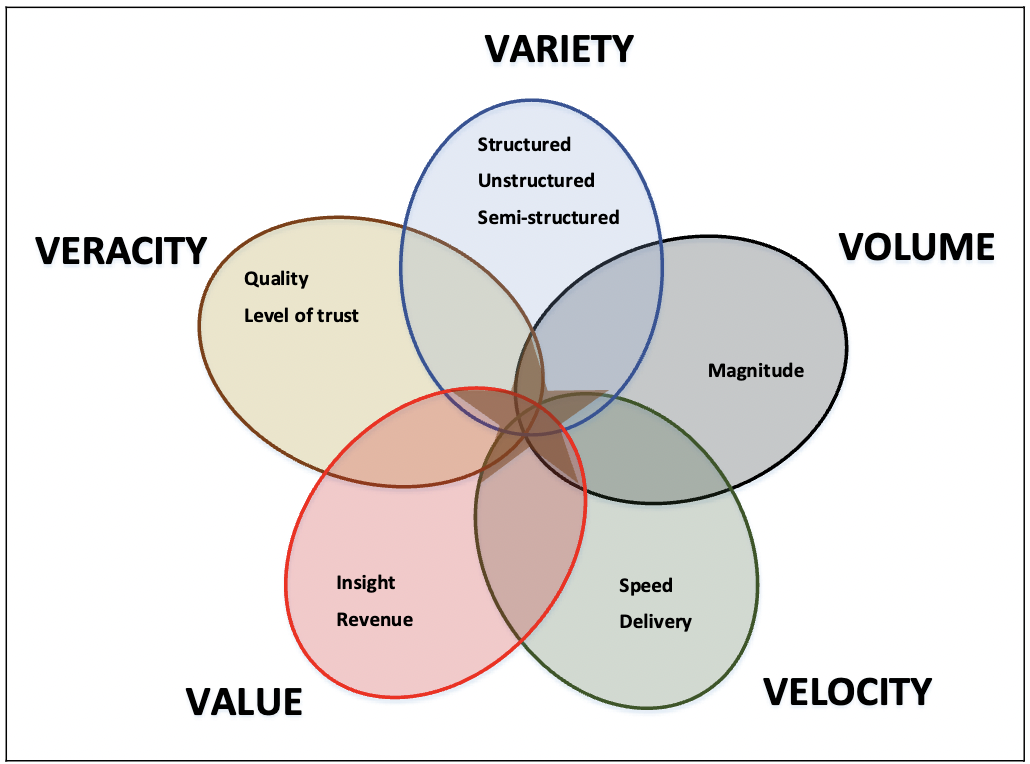
\includegraphics[width=0.8\textwidth]{img/bigdata.png}
    \caption{Mô hình 5V của dữ liệu lớn \cite{Husamaldin2019}}
    \label{fig:bigdata}
    \end{figure}
\vspace*{1ex}
\begin{itemize}
    \item \textbf{Khối lượng (Volume)}: Đề cập đến quy mô dữ liệu cực lớn.
    \item \textbf{Tốc độ (Velocity)}: Tốc độ dữ liệu được tạo ra, truyền tải và xử lý.
    \item \textbf{Tính đa dạng (Variety)}: Nguồn và định dạng dữ liệu đa dạng như văn bản, hình ảnh, video, v.v.
    \item \textbf{Tính xác thực (Veracity)}: Mức độ đáng tin cậy và chất lượng của dữ liệu.
    \item \textbf{Giá trị (Value)}: Tiềm năng khai thác thông tin hữu ích từ dữ liệu.
\end{itemize}

Dữ liệu sinh ra từ các thiết bị \ac{iot} được xem là một trong những nguồn tạo ra dữ liệu lớn (\ac{bd}) quan trọng và phát triển nhanh chóng hiện nay. Với hàng tỷ thiết bị cảm biến, máy móc, thiết bị đeo tay và phương tiện kết nối Internet, lượng dữ liệu được tạo ra mỗi ngày rất lớn, đa dạng về định dạng và tốc độ phát sinh liên tục theo thời gian thực. Dữ liệu \ac{iot} mang đầy đủ các đặc điểm của dữ liệu lớn như: khối lượng (volume) lớn, tốc độ (velocity) cao, tính đa dạng (variety) về loại dữ liệu, mức độ xác thực (veracity) không đồng đều và tiềm năng mang lại giá trị (value) lớn nếu được khai thác hiệu quả. Chính vì vậy, dữ liệu \ac{iot} không chỉ là một phần của dữ liệu lớn mà còn đóng vai trò quan trọng trong việc thúc đẩy nhu cầu phát triển các nền tảng xử lý dữ liệu lớn hiện đại.

\subsection{Các thành phần của Apache Spark}

Trong những năm gần đây, các nền tảng xử lý dữ liệu lớn như Apache Spark đã thu hút sự quan tâm rộng rãi từ cộng đồng nghiên cứu và công nghiệp. Apache Spark là một hệ thống xử lý dữ liệu phân tán quy mô lớn, có khả năng thực thi nhanh các tác vụ trên các cụm dữ liệu lớn. So với Hadoop MapReduce, Spark có thể đạt tốc độ xử lý nhanh hơn khoảng 100 lần trong một số trường hợp nhờ vào khả năng xử lý trong bộ nhớ (\textit{in-memory processing}) \cite{Karau2015}.

Bên cạnh đó, Spark cung cấp giao diện lập trình linh hoạt thông qua các API hỗ trợ nhiều ngôn ngữ phổ biến như Java, Scala, Python và R, giúp việc phát triển và triển khai ứng dụng trở nên thuận tiện hơn.

Apache Spark bao gồm nhiều thành phần chính tạo thành một hệ sinh thái hoàn chỉnh, hỗ trợ đa dạng các tác vụ phân tích dữ liệu như xử lý dữ liệu tuần tự, truy vấn SQL, phân tích luồng dữ liệu thời gian thực, học máy và xử lý đồ thị (Hình~\ref{fig:spark}).

\vspace*{1ex}
    \begin{figure}[ht]
    \centering
    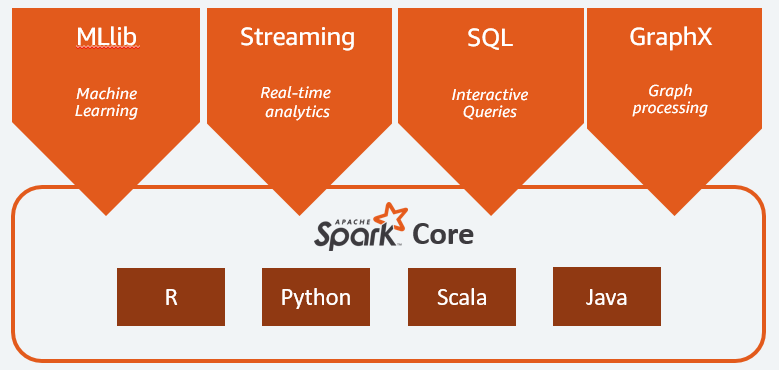
\includegraphics[width=0.8\textwidth]{img/spark.png}
    \caption{Các thành phần của Apache Spark}
    \label{fig:spark}
    \end{figure}
\vspace*{1ex}
Apache Spark bao gồm nhiều thành phần cốt lõi, mỗi thành phần đảm nhận một chức năng cụ thể trong quá trình xử lý dữ liệu lớn:

\begin{itemize}
  \item \textbf{Spark Core}: Thành phần trung tâm của Spark, chịu trách nhiệm quản lý bộ nhớ, lập lịch, xử lý lỗi, phân phối tác vụ và giao tiếp với các hệ thống lưu trữ. Nó cung cấp các API cấp cao cho Java, Scala, Python và R, giúp đơn giản hóa việc xử lý phân tán.

  \item \textbf{MLlib}: Thư viện máy học tích hợp sẵn trong Spark, hỗ trợ huấn luyện và triển khai các mô hình học máy trên quy mô lớn. MLlib cung cấp các thuật toán như phân loại, hồi quy, phân cụm, khai thác mẫu và lọc cộng tác.

  \item \textbf{Spark Streaming}: Công cụ xử lý dữ liệu thời gian thực bằng cách chia dòng dữ liệu thành các lô nhỏ để xử lý tương tự như dữ liệu theo lô. Công cụ này cho phép sử dụng lại mã nguồn và hỗ trợ nhiều nguồn dữ liệu như Kafka, Flume, Twitter, HDFS.

  \item \textbf{Spark SQL}: Thành phần truy vấn dữ liệu phân tán, hỗ trợ ngôn ngữ SQL tiêu chuẩn và HiveQL với hiệu suất cao nhờ tối ưu hóa Catalyst và định dạng cột. Nó hỗ trợ nhiều nguồn dữ liệu như JSON, Hive, Parquet, JDBC, MongoDB, Cassandra.

  \item \textbf{GraphX}: Thư viện xử lý đồ thị phân tán, hỗ trợ biểu diễn, chuyển đổi và phân tích dữ liệu đồ thị. GraphX đi kèm với các thuật toán đồ thị phổ biến như PageRank, Connected Components và nhiều thuật toán phân tích khác.
\end{itemize}

\subsection{Kiến trúc của Apache Spark}
Kiến trúc của Apache Spark được xây dựng theo mô hình master–worker trên nền tảng xử lý phân tán. Thành phần trung tâm là \textbf{Spark Driver}, chịu trách nhiệm điều phối quá trình thực thi ứng dụng, bao gồm việc lên lịch, phân phối tác vụ và giám sát tiến trình. Driver tạo ra một phiên bản logic gọi là \textit{DAG} (Directed Acyclic Graph) để xác định luồng thực thi công việc; tổng quan kiến trúc master--worker được minh họa ở Hình~\ref{fig:spark-structure}.

\vspace*{1ex}
    \begin{figure}[ht]
    \centering
    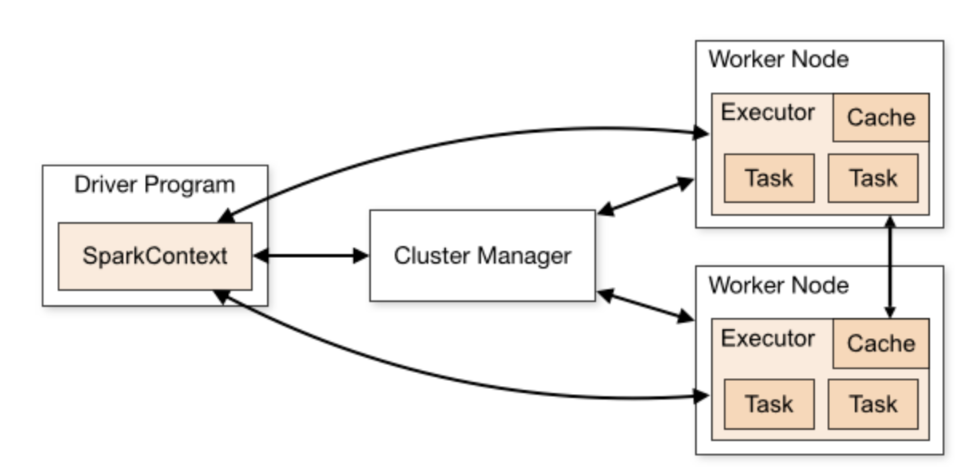
\includegraphics[width=0.85\textwidth]{img/spark-structure.png}
    \caption{Sơ đồ kiến trúc hệ thống Apache Spark}
    \label{fig:spark-structure}
    \end{figure}
\vspace*{1ex}

Các tác vụ được phân phối tới các \textbf{Worker Nodes}, nơi chứa các \textbf{Executor} — tiến trình thực thi thực tế. Mỗi Executor chịu trách nhiệm thực thi các tác vụ (task) và lưu trữ dữ liệu trong bộ nhớ hoặc ổ đĩa nếu cần. Spark sử dụng \textbf{Cluster Manager} (như YARN, Mesos hoặc Standalone) để quản lý tài nguyên trên cụm. Dữ liệu được lưu trữ trên các hệ thống như HDFS, S3, hoặc các cơ sở dữ liệu quan hệ.

\section{Học máy trong phát hiện xâm nhập}

Học máy (\ac{ml}) đã trở thành một công cụ thiết yếu trong việc phát hiện các mẫu tấn công và hành vi bất thường trong lưu lượng mạng \ac{iot}, nhờ khả năng tự động học và thích ứng từ dữ liệu lịch sử \cite{Buczak2016}. Các kỹ thuật học máy phổ biến bao gồm:

\begin{itemize}
\item \textbf{Học có giám sát (Supervised Learning)}: Sử dụng dữ liệu đã được gán nhãn để huấn luyện mô hình phân loại. Một số thuật toán điển hình gồm \ac{rf}, \ac{svm} và Mạng nơ-ron nhân tạo (Neural Networks).
\item \textbf{Học không giám sát (Unsupervised Learning)}: Áp dụng cho các tình huống không có nhãn, tập trung vào việc phát hiện các mẫu bất thường. K-Means là một thuật toán phổ biến trong nhóm này.
\item \textbf{Học tăng cường (Reinforcement Learning)}: Mô hình học dựa trên phản hồi từ môi trường nhằm tối ưu hóa hành vi hoặc quyết định của hệ thống theo thời gian.
\end{itemize}

Trong bối cảnh mạng \ac{iot}, học máy được ứng dụng rộng rãi để phân tích lưu lượng dữ liệu và nhận diện các loại tấn công như DDoS, botnet hay giả mạo gói tin. Theo nghiên cứu của Koroniotis và cộng sự (2020), mô hình \ac{rf} triển khai trên nền tảng Apache Spark đã đạt độ chính xác rất cao khi phát hiện tấn công SYN-DOS, đồng thời đảm bảo tốc độ xử lý cao, phù hợp với yêu cầu thời gian thực của môi trường \ac{iot} \cite{Koroniotis2020}. Tuy nhiên, các kết quả gần như tuyệt đối (xấp xỉ 100\%) trên các tập dữ liệu công khai cần được xem xét thận trọng, vì chúng thường là dấu hiệu của rò rỉ dữ liệu (data leakage) hơn là năng lực thực sự của mô hình. \emph{Rò rỉ dữ liệu} là tình huống trong đó thông tin lẽ ra không sẵn có ở thời điểm triển khai thực tế lại lọt vào quá trình huấn luyện hoặc đánh giá, khiến điểm số bị thổi phồng và không phản ánh đúng khả năng tổng quát hoá của mô hình. Luận văn này nhận diện và xử lý vấn đề đó một cách tường minh ở Chương~\ref{c:thucnghiemdanhgia}.

Tuy nhiên, việc ứng dụng học máy trong hệ thống \ac{iot} vẫn còn gặp nhiều thách thức vì yêu cầu xử lý theo thời gian thực và hạn chế về tài nguyên tính toán. Việc tích hợp học máy với các nền tảng xử lý dữ liệu lớn như Apache Spark mang lại lợi thế đáng kể, giúp xử lý khối lượng dữ liệu lớn với tốc độ cao và hỗ trợ triển khai các thuật toán học máy hiệu quả trong môi trường phân tán.
\subsection{Một số thuật toán học máy}
\begin{itemize}
\item \textbf{Cây quyết định (\ac{dt})} là một trong những thuật toán học máy có giám sát phổ biến, được áp dụng rộng rãi trong các bài toán phân loại. Cấu trúc cơ bản của một cây quyết định bao gồm ba thành phần chính: \textbf{nút gốc}, \textbf{nút quyết định} và \textbf{nút lá}.
Cây quyết định có ưu điểm là dễ hiểu, dễ diễn giải, có thể trực quan hóa và không yêu cầu giả định về phân phối dữ liệu. Tuy nhiên, \ac{dt} cũng dễ bị quá khớp (\textit{overfitting}) nếu không chọn được các tham số hợp lý hoặc xử lý trên dữ liệu nhiễu \cite{mitchell1997machine}.

\item \textbf{Rừng ngẫu nhiên (\ac{rf})} là một thuật toán học máy được sử dụng phổ biến trong cả hai bài toán phân loại và hồi quy. Đây là một kỹ thuật học tập kết hợp (\textit{ensemble learning}) dựa trên việc xây dựng và tổng hợp nhiều cây quyết định độc lập nhằm nâng cao độ chính xác và độ ổn định của mô hình. Thuật toán hoạt động bằng cách tạo ra nhiều cây quyết định trên các tập con khác nhau được chọn ngẫu nhiên từ tập dữ liệu huấn luyện. Mỗi cây được xây dựng dựa trên một mẫu bootstrap (lấy mẫu có hoàn lại), đồng thời tại mỗi nút chia, một tập con ngẫu nhiên của các thuộc tính được chọn để tìm điểm chia tốt nhất, thay vì sử dụng toàn bộ thuộc tính như trong cây quyết định truyền thống \cite{breiman2001random}.

Kết quả cuối cùng được xác định bằng cách:  
\begin{itemize}
    \item Trong bài toán phân loại: lấy kết quả theo nguyên tắc đa số phiếu (\textit{majority voting}) từ các cây.  
    \item Trong bài toán hồi quy: lấy giá trị trung bình từ các dự đoán của từng cây.
\end{itemize}

Việc kết hợp nhiều cây giúp \ac{rf} giảm thiểu hiện tượng quá khớp (\textit{overfitting}) vốn là một nhược điểm thường gặp của các cây quyết định đơn lẻ. Khi số lượng cây trong rừng tăng lên, hiệu suất dự đoán của mô hình có xu hướng ổn định và cải thiện hơn.
\item \textbf{Hồi quy logistic (\ac{lr})} là một phương pháp thống kê được giới thiệu bởi David Cox vào cuối thập niên 1950. Đây là một kỹ thuật học máy có giám sát thường được sử dụng để giải quyết các bài toán phân loại nhị phân, trong đó biến đầu ra (phản hồi) là một biến định tính, nhận giá trị \texttt{0} hoặc \texttt{1}. Mô hình hồi quy logistic cho phép ước tính xác suất xảy ra của một sự kiện cụ thể dựa trên một hoặc nhiều biến đầu vào (độc lập). Một trong những điểm mạnh của phương pháp này là khả năng xác định mức độ ảnh hưởng của từng yếu tố đến xác suất xuất hiện của kết quả, giúp các nhà phân tích hiểu rõ hơn mối quan hệ giữa biến đầu vào và đầu ra \cite{cox1958regression}.

Về mặt toán học, hàm hồi quy logistic được biểu diễn dưới dạng tuyến tính như sau:

\begin{equation}
z_i = \beta_0 + \beta_1 x_{i,1} + \beta_2 x_{i,2} + \cdots + \beta_n x_{i,n}
\label{eq:linear_combination}
\end{equation}

Trong đó:
\begin{itemize}
    \item $x_{i,j}$ là giá trị của biến độc lập thứ $j$ tại quan sát thứ $i$
    \item $\beta_0$ là hệ số chặn (bias), $\beta_j$ là hệ số hồi quy ứng với biến $x_j$
    \item $z_i$ là đầu ra tuyến tính trước khi chuẩn hóa
\end{itemize}

Sau đó, xác suất xảy ra của sự kiện được tính thông qua hàm logistic (sigmoid):
\begin{equation}
P(Y_i = 1 \mid \mathbf{x}_i) = \frac{1}{1 + e^{-z_i}}
\label{eq:sigmoid}
\end{equation}

Trong quá trình huấn luyện, mô hình tìm các hệ số $\beta_j$ tối ưu sao cho hàm mất mát (cross-entropy loss) được tối thiểu hóa.

\item \textbf{\ac{gbt}} là một phương pháp học máy tăng cường (\textit{boosting}) sử dụng các cây quyết định như mô hình học yếu (weak learners). Ý tưởng chính của boosting là xây dựng một mô hình mạnh bằng cách kết hợp nhiều mô hình học yếu được huấn luyện theo trình tự tuần tự. Ở mỗi bước, thuật toán cố gắng giảm thiểu lỗi của mô hình trước bằng cách học từ phần dư (residual) hoặc gradient của hàm mất mát \cite{friedman2001greedy}. Quá trình huấn luyện \ac{gbt} gồm các bước:
\begin{itemize}
    \item Bắt đầu với một mô hình dự đoán ban đầu (thường là giá trị trung bình với bài toán hồi quy).
    \item Tính toán sai số còn lại giữa nhãn thực và dự đoán.
    \item Huấn luyện một cây quyết định để dự đoán phần dư.
    \item Cập nhật mô hình tổng bằng cách cộng mô hình hiện tại với mô hình mới nhân với một hệ số học $\eta$ (learning rate).
\end{itemize}

Giả sử $F_0(x)$ là mô hình khởi tạo ban đầu, mô hình tổng tại bước $m$ được cập nhật theo công thức:

\begin{equation}
F_m(x) = F_{m-1}(x) + \eta \cdot h_m(x)
\end{equation}

Trong đó:
\begin{itemize}
    \item $h_m(x)$ là cây quyết định thứ $m$ học theo gradient của hàm mất mát.
    \item $\eta$ là hệ số học (learning rate), thường $\eta \in (0, 1)$.
\end{itemize}

\item \textbf{\ac{lgbm}} là một framework triển khai thuật toán \ac{gbt}, được phát triển nhằm tối ưu hóa tốc độ huấn luyện và khả năng mở rộng trên các tập dữ liệu lớn \cite{ke2017lightgbm}. Đây là một phương pháp học tập tăng cường (\textit{boosting}) trong đó các cây quyết định được xây dựng tuần tự, mỗi cây mới được huấn luyện để giảm sai số của mô hình trước đó thông qua gradient của hàm mất mát \cite{friedman2001greedy}. 

Giả sử $F_0(x)$ là mô hình khởi tạo ban đầu, mô hình tại bước $m$ được cập nhật như sau:

\begin{equation}
F_m(x) = F_{m-1}(x) + \eta h_m(x)
\end{equation}

Trong đó:
\begin{itemize}
    \item $h_m(x)$ là cây quyết định thứ $m$ học theo gradient của hàm mất mát,
    \item $\eta$ là hệ số học (\textit{learning rate}), thường $\eta \in (0,1)$.
\end{itemize}

Khác với \ac{gbt} truyền thống, \ac{lgbm} sử dụng cơ chế phát triển cây theo hướng leaf-wise thay vì level-wise, đồng thời áp dụng thuật toán histogram-based splitting và kỹ thuật Gradient-based One-Side Sampling (GOSS) nhằm giảm chi phí tính toán và tăng tốc độ huấn luyện. Tuy nhiên, do thư viện gốc của \ac{lgbm} (thông qua SynapseML) chỉ hỗ trợ kiến trúc x86\_64 và không chạy được trên thiết bị biên ARM (Jetson Orin Nano Super) — mục tiêu triển khai của luận văn — nên \ac{lgbm} \emph{không} được đưa vào bộ thuật toán so sánh thực nghiệm; XGBoost và GBT đại diện cho họ gradient boosting.

\item \textbf{\ac{nb}} là một phương pháp phân loại xác suất dựa trên định lý Bayes với giả định độc lập có điều kiện giữa các đặc trưng \cite{mccallum1998comparison}. Mặc dù giả định này thường không hoàn toàn đúng trong thực tế, mô hình vẫn cho hiệu quả tốt trong nhiều bài toán phân loại dữ liệu nhiều chiều.

Theo định lý Bayes:

\begin{equation}
P(y|x) = \frac{P(x|y)P(y)}{P(x)}
\end{equation}

Với giả định độc lập giữa các đặc trưng:

\begin{equation}
P(x|y) = \prod_{i=1}^{n} P(x_i|y)
\end{equation}

Mô hình lựa chọn lớp có xác suất hậu nghiệm lớn nhất:

\begin{equation}
\hat{y} = \arg\max_y P(y)\prod_{i=1}^{n} P(x_i|y)
\end{equation}

Ưu điểm của \ac{nb} là đơn giản, tốc độ huấn luyện nhanh và phù hợp với dữ liệu kích thước lớn; tuy nhiên, hạn chế chính nằm ở giả định độc lập giữa các đặc trưng.

\item \textbf{Support Vector Machine (\ac{svm})} là một thuật toán học có giám sát được đề xuất bởi Cortes và Vapnik \cite{cortes1995support}, nhằm tìm siêu phẳng tối ưu phân tách dữ liệu với khoảng cách biên (margin) lớn nhất. 

Trong trường hợp dữ liệu tuyến tính, bài toán tối ưu được biểu diễn như sau:

\begin{equation}
\min_{w,b} \frac{1}{2} ||w||^2
\end{equation}

với điều kiện:

\begin{equation}
y_i(w \cdot x_i + b) \ge 1
\end{equation}

Trong trường hợp dữ liệu không tuyến tính, \ac{svm} sử dụng kỹ thuật \textit{kernel trick} để ánh xạ dữ liệu sang không gian chiều cao hơn, cho phép phân tách tuyến tính trong không gian mới. Nhờ cơ chế tối ưu hóa chặt chẽ, \ac{svm} thường đạt hiệu suất cao trong các bài toán phân loại với dữ liệu chiều cao.

\item \textbf{Multilayer Perceptron - MLP} là một mô hình học sâu cơ bản gồm nhiều lớp ẩn, có khả năng mô hình hóa các mối quan hệ phi tuyến giữa các đặc trưng \cite{rumelhart1986learning}. 

Mỗi neuron trong mạng thực hiện phép biến đổi tuyến tính:

\begin{equation}
z = w^T x + b
\end{equation}

sau đó áp dụng hàm kích hoạt phi tuyến:

\begin{equation}
a = \sigma(z)
\end{equation}

Trong đó $\sigma(\cdot)$ có thể là các hàm kích hoạt như sigmoid, tanh hoặc ReLU. Quá trình huấn luyện sử dụng thuật toán lan truyền ngược (\textit{backpropagation}) nhằm cập nhật trọng số thông qua tối thiểu hóa hàm mất mát bằng gradient descent. MLP có khả năng biểu diễn mạnh nhưng yêu cầu dữ liệu huấn luyện đủ lớn và quá trình điều chỉnh siêu tham số cẩn thận để tránh hiện tượng quá khớp.

\item \textbf{\ac{xgb}} là một phiên bản cải tiến của thuật toán \ac{gbt} truyền thống, được đề xuất bởi Chen và Guestrin vào năm 2016. \ac{xgb} được thiết kế để tối ưu hóa tốc độ huấn luyện, hiệu suất mô hình, và khả năng xử lý dữ liệu quy mô lớn trong các hệ thống tính toán phân tán \cite{chen2016xgboost}. \ac{xgb} sử dụng các chiến lược sau để cải thiện hiệu năng:
\begin{itemize}
    \item Ánh xạ gradient và Hessian để tối ưu hóa hiệu quả (second-order optimization).
    \item Cắt tỉa cây (pruning) theo độ phức tạp thay vì độ sâu cố định.
    \item Tính song song trong việc tìm điểm chia tối ưu (split finding).
    \item Hỗ trợ xử lý thiếu giá trị (missing values) tự động.
\end{itemize}

Mô hình \ac{xgb} đã được ứng dụng thành công trong nhiều bài toán học máy thực tế như dự báo tài chính, chẩn đoán y tế, phát hiện gian lận và phân tích hành vi khách hàng, nhờ độ chính xác cao và hiệu quả tính toán tốt.
\end{itemize}
\subsection{Một số thuật toán Ensemble learning}
\textbf{Ensemble Learning (\ac{el})} là một kỹ thuật trong học máy nhằm kết hợp nhiều mô hình riêng lẻ để nâng cao độ chính xác và độ ổn định trong dự đoán. Thay vì chỉ dựa vào một mô hình đơn lẻ, phương pháp \ac{el} tận dụng sức mạnh tổng hợp của nhiều mô hình — ví dụ như \ac{dt}, \ac{rf}, \ac{lr}, v.v. --- để xây dựng một hệ thống dự đoán chính xác hơn. Nguyên lý cốt lõi của \ac{el} là: mỗi mô hình riêng lẻ có thể chỉ đạt độ chính xác thấp hoặc dự đoán sai ở một số trường hợp, nhưng sự kết hợp hợp lý của chúng có thể giảm thiểu sai số, tăng độ chính xác nhờ tận dụng điểm mạnh và khắc phục điểm yếu của từng mô hình thành phần \cite{zhou2012ensemble}.

Kỹ thuật \ac{el} đã chứng minh được tính hiệu quả cao trong nhiều lĩnh vực yêu cầu độ chính xác cao như: phát hiện gian lận, phân tích dữ liệu lớn, nhận diện hình ảnh và xử lý ngôn ngữ tự nhiên. Trong lĩnh vực bảo mật mạng \ac{iot}, \ac{el} cũng được ứng dụng để cải thiện khả năng phát hiện bất thường hoặc xâm nhập dựa trên nhiều mô hình học máy được huấn luyện song song hoặc tuần tự.

Một số phương pháp phổ biến của \ac{el} bao gồm:
\begin{itemize}
    \item \textbf{Voting}: Với bài toán phân loại, mỗi mô hình con bỏ phiếu cho một lớp và lớp có số phiếu cao nhất sẽ là đầu ra cuối cùng (đa số phiếu hoặc trung bình xác suất). Các bước của voting được mô tả chi tiết ở Thuật toán~\ref{voting_ag1}.
    \item \textbf{Boosting}: Huấn luyện các mô hình tuần tự, trong đó mỗi mô hình mới tập trung vào các mẫu mà mô hình trước đã dự đoán sai (ví dụ: \ac{gbt}, AdaBoost, \ac{xgb}). Các bước của boosting được mô tả chi tiết ở Thuật toán~\ref{boosting_ag1}.
    \item \textbf{Bagging (Bootstrap Aggregating)}: Huấn luyện nhiều mô hình trên các tập con ngẫu nhiên (lấy mẫu có hoàn lại) của tập dữ liệu gốc, sau đó tổng hợp kết quả dự đoán (ví dụ: Random Forest). Các bước của bagging được mô tả chi tiết ở Thuật toán~\ref{bagging_ag1}.
\end{itemize}

\ac{el} đặc biệt hữu ích trong các hệ thống phát hiện xâm nhập (\ac{ids}) vì cần phân tích lượng lớn dữ liệu phức tạp, và việc kết hợp nhiều mô hình có thể giúp tăng khả năng phát hiện các gói tin bất thường mà một mô hình đơn lẻ có thể bỏ sót.

\begin{algorithm}[htbp]
\caption{Voting: Kết hợp dự đoán từ nhiều mô hình phân loại}
\label{voting_ag1}
\textbf{Đầu vào:}
\begin{itemize}
  \item Tập huấn luyện $\mathcal{D} = \{(x_i, y_i)\}_{i=1}^N$
  \item Tập mô hình phân loại cơ sở $M_1, M_2, \dots, M_K$
  \item Kiểu voting: \texttt{HARD} hoặc \texttt{SOFT}
\end{itemize}

\textbf{Đầu ra:} Nhãn dự đoán cuối cùng $y_{\text{vote}}$ cho điểm dữ liệu $x$

\begin{algorithmic}[1]
\State \textbf{Khởi tạo:} danh sách $S = \{\}$ \Comment{Lưu dự đoán hoặc xác suất}
\If{voting = \texttt{HARD}}
    \For{$j = 1$ to $K$}
        \State $y_j \gets M_j(x)$ \Comment{Dự đoán nhãn của mô hình thứ $j$}
        \State Thêm $y_j$ vào $S$
    \EndFor
    \State $y_{\text{vote}} \gets$ nhãn xuất hiện nhiều nhất trong $S$
\ElsIf{voting = \texttt{SOFT}}
    \State Khởi tạo xác suất tổng $P_{\text{sum}}[c] = 0, \forall c \in \{1, \dots, C\}$
    \For{$j = 1$ to $K$}
        \State Lấy xác suất $P_j(y = c \mid x)$ từ mô hình $M_j$
        \For{mỗi lớp $c = 1$ to $C$}
            \State $P_{\text{sum}}[c] \gets P_{\text{sum}}[c] + P_j(y = c \mid x)$
        \EndFor
    \EndFor
    \State $y_{\text{vote}} \gets \arg\max_{c} P_{\text{sum}}[c]$
\EndIf
\State \Return $y_{\text{vote}}$
\end{algorithmic}
\end{algorithm}

\begin{algorithm}[htbp]
\caption{Boosting: Học tăng cường tuần tự}
\label{boosting_ag1}
\textbf{Đầu vào:}
\begin{itemize}
  \item Tập dữ liệu huấn luyện $\mathcal{D} = \{(x_i, y_i)\}_{i=1}^N$
  \item Số lượng vòng lặp (mô hình yếu): $T$
\end{itemize}

\textbf{Đầu ra:} Mô hình tăng cường $F_T(x)$

\begin{algorithmic}[1]
\State \textbf{Khởi tạo:} $F_0(x) \gets 0$ \Comment{Mô hình khởi đầu có thể là 0 hoặc dự đoán trung bình}
\For{$t = 1$ to $T$}
    \State Tính phần dư (residuals) cho từng mẫu: $r_i^{(t)} = y_i - F_{t-1}(x_i)$
    \State Huấn luyện mô hình yếu $h_t(x)$ trên các phần dư $r_i^{(t)}$
    \State Cập nhật mô hình: $F_t(x) = F_{t-1}(x) + \eta \cdot h_t(x)$
\EndFor
\State \Return $F_T(x)$
\end{algorithmic}
\end{algorithm}

\begin{algorithm}[htbp]
\caption{Bagging: Bootstrap Aggregating}
\label{bagging_ag1}
\textbf{Đầu vào:}
\begin{itemize}
  \item Tập huấn luyện $\mathcal{D} = \{(x_i, y_i)\}_{i=1}^N$, với $x_i \in \mathbb{R}^d$, $y_i \in \{1, 2, \dots, C\}$
  \item Số lượng mô hình cơ sở: $K$
\end{itemize}

\textbf{Đầu ra:} Dự đoán cuối cùng $y_{\text{bag}}$ cho một điểm dữ liệu $x$

\noindent
\begin{algorithmic}[1]
\State \textbf{Khởi tạo:} Danh sách mô hình $M_1, M_2, \dots, M_K$

\For{$k = 1$ to $K$}
  \State Tạo mẫu bootstrap $\mathcal{D}^{(k)}$ từ $\mathcal{D}$ (lấy mẫu ngẫu nhiên có hoàn lại)
  \State Huấn luyện mô hình $M_k \gets \text{Train}(\mathcal{D}^{(k)})$
\EndFor

\State \textbf{Khởi tạo:} Danh sách dự đoán $Y = \{\}$

\For{$k = 1$ to $K$}
  \State Thực hiện dự đoán $y_k \gets M_k(x)$
  \State Thêm $y_k$ vào $Y$
\EndFor

\State Tính $y_{\text{bag}} \gets \text{Voting}(Y)$ \Comment{Hard voting hoặc trung bình xác suất nếu dùng soft}

\State \Return $y_{\text{bag}}$
\end{algorithmic}
\end{algorithm}

\pagebreak
